\section{Animal-10N transfer and independent replications}
\label{sec:animalpilot}
The Animal-10N experiment transfers the CIFAR recipe without tuning it to Animal test outcomes. Base 42 was the technical pilot; bases 43 and 44 were planned before fitting the pilot and were subsequently run with the same settings regardless of the pilot's favorable sign. All three runs retain the frozen protocol file byte-for-byte, 50 training epochs, a fixed 45,000/5,000 observed-label train/validation partition, three nested head seeds, and unchanged target and policy grids. The minimum noisy-validation cross entropy occurs at zero-based epochs 2, 1, and 2 respectively. Thus the experiment contains three independently initialized bases, not nine base replications or three independently resampled dataset splits.

The data realization is an explicitly identified public Activeloop mirror of Animal-10N~\citep{song2019selfie}, with 50,000 training and 5,000 test RGB $64\times64$ images. Repacking preserves decoded pixels, stored labels and train/test membership; IDs follow mirror row order. Original KAIST IDs/order and equality to the original archive are not independently verified. All runs record the same supplied-file hashes and saved source provenance. Complete clean training labels are unavailable; training-noise detection metrics are not reported.

\begin{table}[t]
\centering
\small
\begin{tabular}{lrrrrr}
\toprule
Method & Base42 & Base43 & Base44 & Mean & Error AUROC \\
\midrule
Base FP32 & 89.24 & 88.80 & 89.18 & 89.07 & 0.9079 \\
Uniform TTA & 89.56 & 89.86 & 89.92 & 89.78 & 0.9079 \\
MSP & 89.82 & 89.88 & 89.82 & 89.84 & 0.9079 \\
Static & 89.61 & 89.96 & 89.92 & 89.83 & 0.8954 \\
Augmented static & 89.68 & 89.89 & 89.92 & 89.83 & 0.8927 \\
History-50 & 89.95 & 90.22 & 89.91 & 90.03 & 0.8202 \\
Early-5 & 90.11 & 90.01 & 89.96 & 90.03 & 0.9091 \\
\bottomrule
\end{tabular}

\caption{Animal-10N accuracy (\%) by independent base and equal-base mean, followed by mean original-view base-error AUROC. Learned rows first average three heads within each base. Every method selects its own budget and temperature on noisy validation.}
\label{tab:animalpilot}
\end{table}

\paragraph{Accuracy gains attenuate in replication.}
Early-5 obtains 90.03\% averaged equally over bases, compared with 89.07\% for the matched downstream FP32 bases and 89.78\% for selected uniform TTA. The mean gains are 0.96 and0.25 percentage points. The TTA advantage by base is 0.55, 0.15, and 0.04 points; its between-base sample SD is0.27 points, not a confidence interval. Five of nine nominal conditional head-level paired intervals against selected TTA strictly exclude zero. One Early-5 head on base 43 is below TTA in point accuracy. These results preserve a positive within-base mean in each run but show a weaker and less consistent effect than the first pilot alone suggested.

\paragraph{Static and full-history controls.}
The augmentation-matched static control averages 89.83\%, a 0.20-point mean Early-5 advantage. Only two of nine conditional accuracy intervals strictly exclude zero, one touches zero and six cross zero. All nine corresponding original-view error-AUROC difference intervals are positive. History-50 averages 90.0267\%, versus 90.0289\% for Early-5: their 0.0022-point difference is negligible at the displayed precision. No paired Early-5 accuracy interval against History-50 is strictly positive; one on base 43 strictly favors History-50 and eight cross zero. Consequently the transfer results do not establish a general accuracy advantage of Early-5 over a full-history scalar summary or the matched augmentation control.

\paragraph{Reliability and calibration are not uniformly improved.}
Mean original-view base-error AUROC is 0.9091 for Early-5 versus 0.9079 for MSP, but the per-base comparisons are 0.9131 versus 0.9014, 0.9083 versus 0.9128, and 0.9059 versus 0.9095. The two replication bases therefore reverse the pilot's AUROC improvement over MSP. Early-5 remains above the learned static/history controls in this ranking metric, which does not imply dominance over the simpler MSP baseline. Mean NLL improves relative to the base on all three runs, from 0.3367 to 0.3227 overall; mean-head ECE worsens on every base, from 0.0419 to 0.0527 overall.

\paragraph{Execution and verification limits.}
All four stages report completion for all bases in 2.70, 2.67, and 2.89 hours respectively on two Tesla T4 GPUs per session. These are measured wall times, not GPU-hour quota charges or replicated inference benchmarks. Base training-loop AMP accuracies are 89.28\%, 88.82\%, 89.16\%; matched downstream FP32 accuracies are 89.24\%, 88.80\%, 89.18\%. The paths remain separate rather than mixing base measurements. A subsequent CPU replay on the three full Kaggle Outputs verifies dataset bytes, sample IDs and labels, minimum-validation checkpoints, frozen validation choices, all 21 scalar heads per base on their saved projected features, 40 selected result rows per base, and the reported paired intervals. All three bases pass the recorded-cache checks; the numerical replay takes 199.34 seconds excluding environment setup. Base weights additionally reproduce probabilities on eight fixed validation images per base, with maximum absolute differences below $1.2\times10^{-6}$. Full feature extraction and PCA fitting are not rerun, so this check does not independently reconstruct the complete training pipeline. No settings or policies were changed during replay.

\begin{figure}[t]
\centering
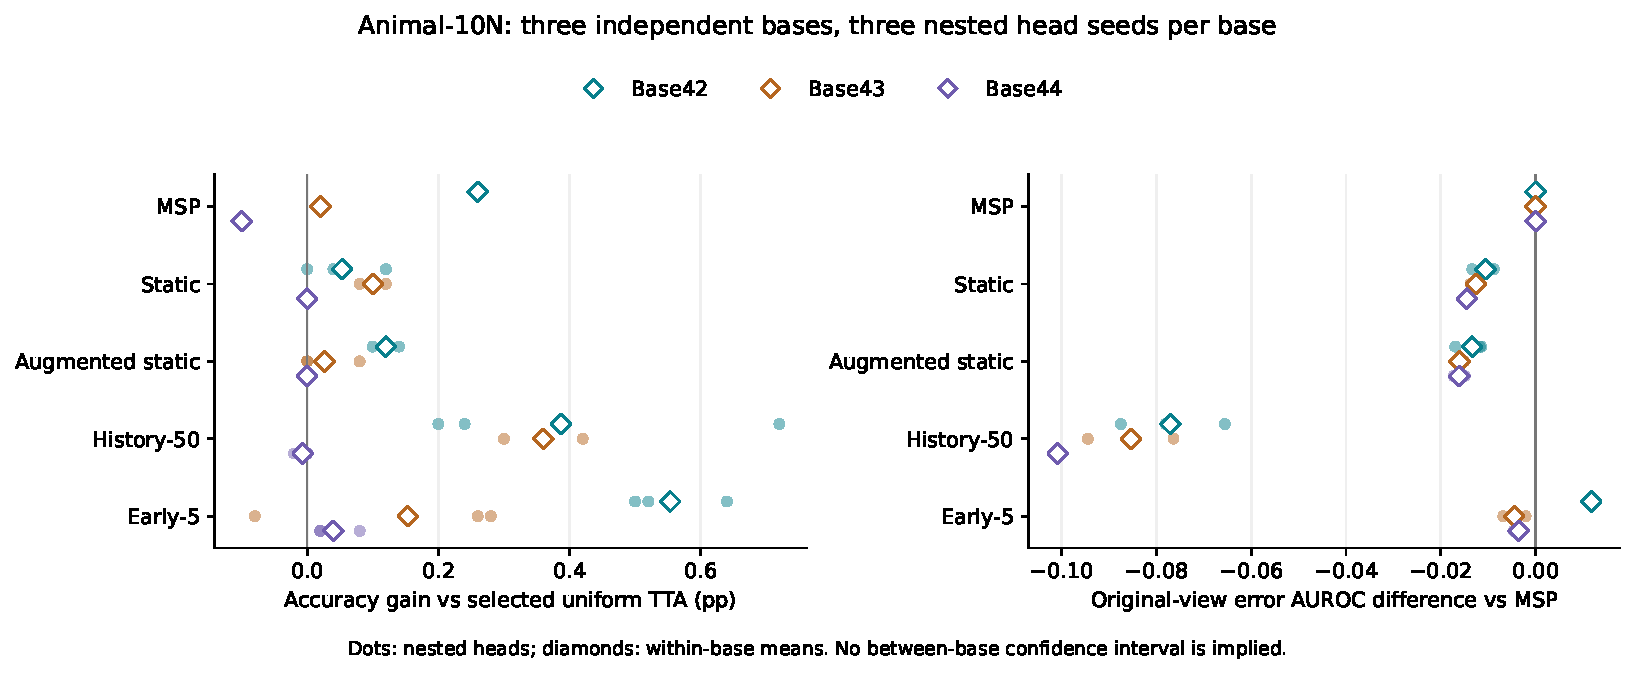
\includegraphics[width=\linewidth]{figures/animal10n_replications.pdf}
\caption{Animal-10N transfer across three independent base initializations. Dots show nested heads, diamonds within-base means and colors base seeds. Left: accuracy relative to each base's validation-selected uniform TTA. Right: error-ranking AUROC relative to original-view MSP. There is no implied confidence interval across independent bases.}
\end{figure}
